\begin{figure*}
    \centering
    \begin{subfigure}[t]{0.195\textwidth}
        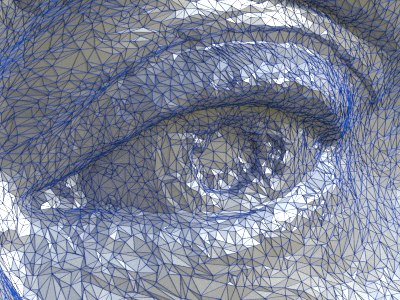
\includegraphics[width=\textwidth]{process_f02_01}
        \caption{Original 3D head scan data: 1.4 million polys}
        \label{fig:process_original_scan}
    \end{subfigure}
    \hfill
    \begin{subfigure}[t]{0.195\textwidth}
        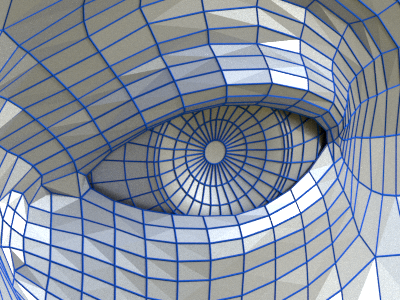
\includegraphics[width=\textwidth]{process_f02_02}
        \caption{Retopologized head model: 9 thousand polys}
        \label{fig:process_retopo}
    \end{subfigure}
    \hfill
    \begin{subfigure}[t]{0.195\textwidth}
        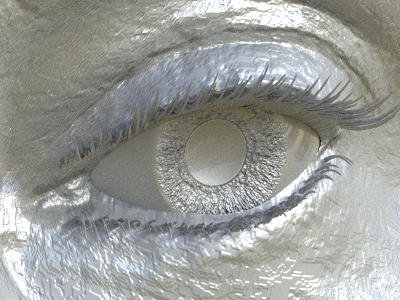
\includegraphics[width=\textwidth]{process_f02_03}
        \caption{Surface detail is stored in displacement maps}
        \label{fig:process_displaced_subdiv}
    \end{subfigure}
    \hfill
    \begin{subfigure}[t]{0.195\textwidth}
        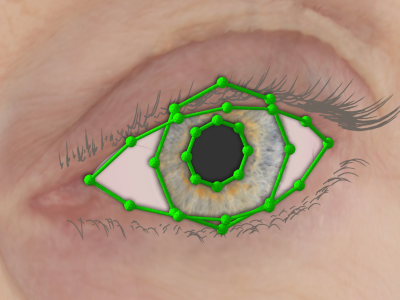
\includegraphics[width=\textwidth]{process_f02_04}
        \caption{3D iris and eyelid landmarks are annotated}
    \end{subfigure}
    \hfill
    \begin{subfigure}[t]{0.195\textwidth}
        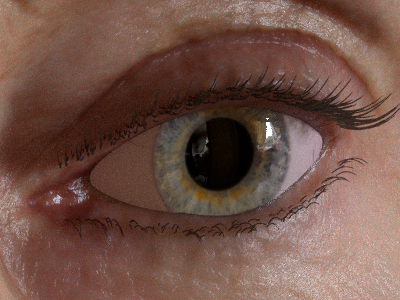
\includegraphics[width=\textwidth]{process_f02_05}
        \caption{The final render}
    \end{subfigure}
    \caption{Model preparation process}
    \label{fig:process}
\end{figure*}